%%%%%%%%%%%%%%%% Präambel-ANFANG
% Die folgenden Zeilen zwischen Präambel-ANFANG und Präambel-ENDE bitte nicht ändern.

% Das Latex-Dokument beginnt mit dem \documentclass-Befehl, welcher eine angepasste Version der ACM sig-alternate-Klasse (ewks-latex) referenziert. Die Datei ewks-latex.cls muss sich im gleichen Verzeichnis wie die Zusammenfassung befinden.
\documentclass[ngerman]{ewks-latex}

% Anpassungen an die deutsche Sprache.
\usepackage[ngerman]{babel}

% Angaben zu Zeichensätzen (unter anderem ist Nutzung deutscher Umlaute möglich).
\usepackage[T1]{fontenc}
\usepackage[utf8]{inputenc}

% Entfernung von für den Copyright-Hinweis der Konferenz reserviertem Platz in der ersten Spalte.
\usepackage{etoolbox}
\makeatletter
\patchcmd{\maketitle}{\@copyrightspace}{}{}{}
\makeatother

% Anzahl der Autoren der Zusammenfassung (in diesem Semester zwei Studenten).
\numberofauthors{2}

%%%%%%%%%%%%%%%%%%%%%%%%%%%%%%%%%%%%%%%%%%%%%%%%%%%%%%%%%%%%%%%%%%%%%%%%%%%%%%%%%%%%%%%%%%%%%%%%
% Zusätzlich benötigte Packages
% Ohne dieses Package können keine eps Bilder angezeigt werden.
\usepackage{epstopdf}
%
% Ohne Color kann der Text nicht eingefärbt werden.
\usepackage{color}
%
% Ohne graphicx können keine Bilder eingebunden werden.
\usepackage{graphicx}
%
% Ohne verbatim können keine Mehrzeiligen Kommentare genutzt werden.
\usepackage{verbatim}
%
% Möglichkeit Bilder zu fixieren.
\usepackage{float}
% URLs mit \url{} In das Dokument einfügen
\usepackage{hyperref}
%%%%%%%%%%%%%%%%%%%%%%%%%%%%%%%%%%%%%%%%%%%%%%%%%%%%%%%%%%%%%%%%%%%%%%%%%%%%%%%%%%%%%%%%%%%%%%%%

%%%%%%%%%%%%%%%%%%%%%%%%%%%%%%%%%%%%%%%%%%%%%%%%%%%%%%%%%%%%%%%%%%%%%%%%%%%%%%%%%%%%%%%%%%%%%%%%
% Command für TODOs 
% Bsp:
%	\todo{<name>}{<was muss gemacht werden>}
\newcommand{\todo}[2]{\textcolor{red}{\underline{\textbf{TODO [#1]}} \\ #2}}
%%%%%%%%%%%%%%%%%%%%%%%%%%%%%%%%%%%%%%%%%%%%%%%%%%%%%%%%%%%%%%%%%%%%%%%%%%%%%%%%%%%%%%%%%%%%%%%%

%%%%%%%%%%%%%%%%%%%%%%%%%%%%%%%%%%%%%%%%%%%%%%%%%%%%%%%%%%%%%%%%%%%%%%%%%%%%%%%%%%%%%%%%%%%%%%%%
% Command für lstListings mit Code. Muss mit "\end{lstlisting}" beendet werden
% Bsp:
%	\lstlistingCode{Titel bzw. Beschriftung} 
%	<QuellCode> 
%	\end{lstlisting}
\newcommand{\lstlistingCode}[2]{\begin{lstlisting}[caption=#1, label=lst:#2, language=java, basicstyle=\small, tabsize=4,frame=single, showstringspaces=false, numbers=left, keywordstyle=\bfseries]}
%%%%%%%%%%%%%%%%%%%%%%%%%%%%%%%%%%%%%%%%%%%%%%%%%%%%%%%%%%%%%%%%%%%%%%%%%%%%%%%%%%%%%%%%%%%%%%%%


%%%%%%%%%%%%%%%% Präambel-ENDE

% Das lipsum-Paket wird für die Generierung von Blindtext in dieser Beispieldatei verwendet und kann aus der tatsächlichen Abgabe entfernt werden.
\usepackage{lipsum}

% Das listings-Paket kann zum Setzen von Quellcode verwendet werden. Es kann auch entfernt werden, falls kein Quellcode gesetzt werden muss.
\usepackage{listings}

% Start des Dokuments.
\begin{document}

% Angabe des *englischen* Titels des Papers.
% Bitte das Tag Approach to Define Highly Scalable Metamodels Based on JSON entsprechend ersetzen.
\title{Approach to Define Highly Scalable Metamodels Based on JSON}

% Als Untertitel sollte darauf hingewiesen werden, dass es sich um eine Zusammenfassung des Papers der jeweiligen Konferenz inkl. Jahrgang handelt.
% Bitte das Tag 2015 entsprechend ersetzen.
\subtitle{Zusammenfassung des auf der BigMDE 2015 veröffentlichten, gleichnamigen Papers}

% Angaben zu den Autoren der *Zusammenfassung*.
% Bitte die Tags <VORNAMEx>, <NAMEx>, <MATRIKELNRx>, <EMAILx> durch die eigenen Angaben ersetzen.
\author{
	% Erster Autor (i. d. R. der Corresponding Author, der auch die Mail zur Gruppenanmeldung und Papier-Auswahl verfasst hat).
	\alignauthor
	<Peter> <S>\\
	\affaddr{Fachhochschule Dortmund, Fachbereich Informatik}\\
    \affaddr{<MATRIKELNR1>}\\
    \email{ps@fh-dortmund.de}    
	% Zweiter Autor (diese Kommentarzeile nicht entfernen!)
	\alignauthor
	Sascha D\"upre\\
	\affaddr{Fachhochschule Dortmund, Fachbereich Informatik}\\
    \affaddr{7075071}\\
    \email{saschad@stud.fh-dortmund.de}    
}

% Titel setzen. Dieser Befehl sollte an dieser Stelle belassen werden und vor dem eigentlichen Text auftauchen.
\maketitle

% Das Paper wie auch die Zusammenfassung gliedern sich in mehrere Abschnitte (\section-Befehl). Der erste Abschnitt sollte der Einleitung (Introduction) vorbehalten sein und eine Spalte nicht überschreiten.


\section{Einleitung}
Das Paper \textit{\glqq Approach to Define Highly Scalable Metamodels Based on JSON\grqq}\cite{gerhart2015approach} wurde im Rahmen der BigMDE 2015 veröffentlicht und beschreibt die Gestaltung für einen neuen Ansatz zur Speicherung von \textbf{D}omain-\textbf{S}pecific \textbf{M}odeling \textbf{L}anguages (DSMLs). \\
DSMLs werden in der Softwareentwicklung eingesetzt, um aus verschiedenen Diagrammen Quelltext zu generieren. Alternativ können aber auch aus textuellen Inhalten Diagramme generiert werden, um sie so übersichtlicher und verständlicher zu machen. Hiermit gemeint ist beispielsweise die Generierung eines Klassendiagramms zu einem dazugehörigen Java-Programm. Dies kann entweder durch den Quellcode an sich geschehen oder durch spezielle \textit{@Annotationen} die im Quellcode gesetzt werden müssen \cite{france2005domain}. \\
Zur Speicherung dieser Diagramme wurde in der Vergangenheit oft auf XML zurückgegriffen. Für Modelle die mit wenigen Knoten und Kanten auskommen ist dies unproblematisch. In großen Modellen ist die Anzahl der beiden Elemente aber unter Umständen so hoch, dass die angelegten XML-Dateien mehrere Gigabyte Speicher beanspruchen.\\ 
Neben dem großen Speicherbedarf kommt hier ein Nachteil der dem XML-Format geschuldet ist zum tragen. Modelle können nur als Ganzes geladen bzw. ausgelesen werden. Ein streaming ist somit nicht möglich und die Betrachtung von Teilen des Modells erfordert das Laden des Gesamtmodells. Somit sind diese Modelle nicht skalierbar im Bezug auf ihren Speicherbedarf. Diese Limitierungen der Skalierbarkeit können durch das JSON-Format verbessert und zum Teil sogar aufgehoben werden. Beispielsweise kann der Speicherbedarf durch einen geringeren Overhead im Quellcode reduziert werden und die Modelle können über sogenannte \textit{Identifier} partiell geladen werden. \\
Um die zuvor getroffenen Aussagen zu untermauern und die Vorteile des JSON-Formats faktisch darzustellen wird im Folgenden eine JSON-DSML-Implementierung beschrieben und in einem anschließenden Benchmark mit Ecore verglichen. \\
Die Gliederung dieser Zusammenfassung orientiert sich am Originalpaper \cite{gerhart2015approach}. An einigen Stellen in dieser Zusammenfassung befinden sich Einschübe, um das im Original vorgestellte Metamodell MoDiGen genauer zu beschreiben oder um Hintergründe für Design-Entscheidungen zu verständlicher und durchschaubarer zu machen. 



%Dabei geht es nicht um eine gut lesbare und verständliche Übersicht, sondern um die Generierung der Diagramme. Hierbei gibt es verschiedene Ansätze zur Generierung.

\section{Related Work}
Es gibt verschiedene Metamodelle wie beispielsweise Ecore, \textbf{G}eneric \textbf{M}odeling \textbf{E}nvironment (GME) \cite{ledeczi2001generic} und WebGME \cite{maroti2014online}. Jedes dieser Modelle speichert Kanten als ein Teil der dazugehörigen Knoten. Im beispielhaften Falle eines UML-Klassendiagramms bedeutet das, dass Referenzen in den jeweiligen Klassen gespeichert werden. Diese Methode führt dazu, dass es zu sogenannten Memory Heaps kommt. \\
\textit{Ein Memory Heap ist ein problematisches Speicherphänomen, bei dem der Speicher durch seine Struktur und seine abhängigen Elemente belegt wird. Das bedeutet, dass keine Teile des Speichers freigegeben werden können, obwohl eigentlich nur ein kleiner Teil dieses Speichers tatsächlich genutzt wird. \url{https://pubs.vmware.com/vfabric52/index.jsp?topic=/com.vmware.vfabric.em4j.1.2/em4j/conf-heap-management.html}} \\
Im Bezug auf das Klassendiagramm bedeutet dies, dass bei einer Klasse mit vielen Referenzen jede einzelne Referenz im Speicher vorgehalten werden muss. Das hier aufgeführte Phänomen wird an anderer Stelle aufgegriffen und genauer erläutert \cite{scheidgen2013reference}. Ein Ansatz dieses Problem zu umgehen ist Knoten und Referenzen bzw. Kanten in eigenständig zu speichern. \\
Das Problem das Modelle nicht partiell geladen werden können ist dem XML-Format geschuldet. Hier wurden an anderer Stelle schon Grundvoraussetzungen diskutiert und zu einem Kriterienkatalog zusammengefasst, um Modelle teilweise zu laden \cite{kolovos2013research}. Das JSON-Format erfüllt nicht alle Kriterien dieses Katalogs, bietet aber eine erste Grundlage von der aus weiter entwickelt werden kann.

\section{Ecore Metamodell}
In \cite{gerhart2015approach} wird an vielen Stellen ein Bezug zu Ecore hergestellt, besonders im Rahmen der Evaluation. Damit diese Bezüge und Vergleiche zwischen MoDiGen und Ecore anschaulicher werden wird in diesem Abschnitt ein Überblick über Ecore eingeschoben. Er beinhaltet einen Ausschnitt aus der Architektur des Ecore-Modells, der im Zusammenhang mit dem Originalpaper besonders relevant ist.

\subsection{Architektur}
Der zugrundeliegende Aufbau des Ecore-Modells bildet weitaus mehr modellierungs Möglichkeiten ab, als der Aufbau von MoDiGen (siehe dazu \cite{eclipse_ecore}). Dazu gehören u.a. Pakete (EPackage), Operationen mit Parametern (EOperation, EParameter) und EFactory durch die sich Instanzerzeugungen oder Konvertierungen modellieren lassen. Diese Bestandteile des Ecore-Modells werden bei der folgenden Betrachtung ausgelassen, da sie keinen Beitrag zum Verständnis der Evaluation  leisten. Daher stellt die Abbildung \ref{fig:emf-ecore-kd} lediglich einen Auszug aus dem vollständigen Modell dar und soll die folgenden Ausführungen unterstützen.\\
\\
Die Klasse \texttt{EClass} hat einen Namen und besitzt Attribute \texttt{EAttribute} und Referenzen \texttt{EReference}, die durch Assoziationen modelliert sind. Die Referenz ist über eine Komposition modelliert und kann nicht ohne eine zugeordnete Klasse existieren. Eine abstrakte Klasse \texttt{ETypedElement} die von \texttt{EStructuralFeature} geerbt wird enth\"alt Attribute wie \textit{upper-} und \textit{lowerBound}, durch die sich Multiplizitäten festlegen lassen. \texttt{EStructuralFeature} wird von \texttt{EReference} und \texttt{EAttribute} geerbt. Der Datentyp eines Attributes wird durch eine Assoziation zu \texttt{EDataType} festgelegt. Ecore definiert 21 Java Datentypen, wie u.a. \texttt{EBoolean}, \texttt{EByte} und \texttt{EChar} sowie 10 zus\"atzliche (u.a. \texttt{EDate} und \texttt{EEList}). Das Modell ist unter \cite{eclipse_ecore} vollst\"andig einzusehen.

\begin{figure}
\centering
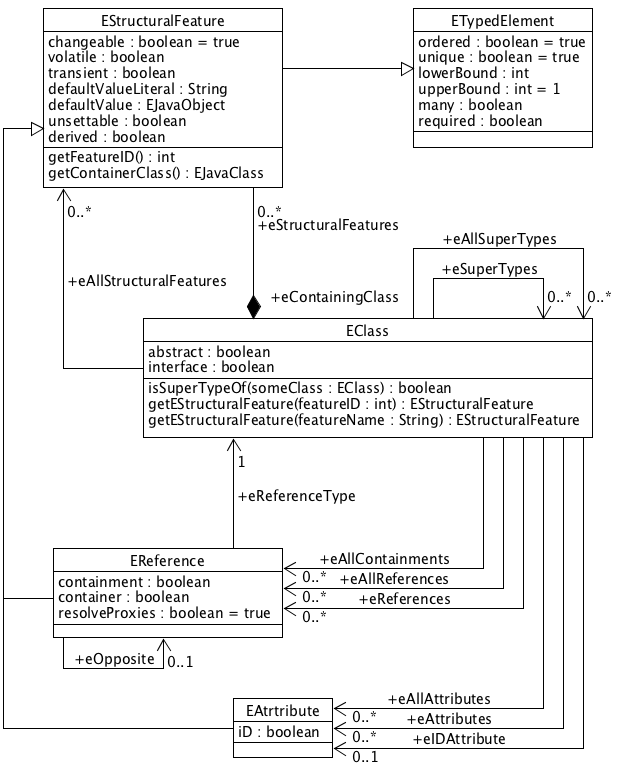
\includegraphics[width=\linewidth]{Abschnitte/Abbildungen/Grafiken/EMF}
\caption{Auschnitt aus dem Ecore-Metamodell des Eclipse Modelling Frameworks \cite{eclipse_ecore}}
\label{fig:emf-ecore-kd}
\end{figure}


Das Listing \ref{lst:ecore-modell} zeigt wie die Klasse \texttt{Female} aus Abbildung \ref{fig:Family-Tree-Model} als Ecore-Modell in XML abgespeichert wird. Die Referenzen \textit{isWife} und \textit{isMother} werden durch \texttt{eStructuralFeatures} mit dem XML-Typ \textit{ecore:EReference} als Kindelemente beschrieben. Die entsprechenden Attribute wie \textit{eType} und \textit{upperBound} sind als XML-Attribute von \texttt{eStructuralFeatures} vermerkt.

\begin{lstlisting}[caption=Auszug der Klasse Female aus Abbildung \ref{fig:Family-Tree-Model} als ECore in XML, label=lst:ecore-modell, language=xml, basicstyle=\small, tabsize=4,frame=single, showstringspaces=false, numbers=left, keywordstyle=\bfseries, breaklines=true]
[...]
  <eClassifiers xsi:type="ecore:EClass" name="Female" eSuperTypes="#//Person">
    <eStructuralFeatures xsi:type="ecore:EReference" name="isWife" eType="#//Male"/>
    <eStructuralFeatures xsi:type="ecore:EReference" name="isMother" upperBound="-1" eType="#//Person"/>
  </eClassifiers>
[...]
\end{lstlisting}


\section{Vorgehensweise}
In diesem Abschnitt wird der Ansatz erkl\"art, indem die Architektur des Metamodells erl\"autert und um ein Beispiel erg\"anzt wird.

\subsection{Architektur}
Die MoDiGen Metamodell-Architektur (Abbildung \ref{fig:MoDiGen-Metamodel}) wurde mit dem Fokus auf Allgemeingültigkeit und Erhalt der bla-Einfachheit- entworfen. Erstellte Modelle werden -- einschließlich der Instanzen -- in standard konformen JSON gespeichert. Dadurch bietet MoDiGen eine sprachunabhängige Modellierung, sowie ein erhöhtes Maß an Skalierbarkeit gegenüber ECore (Absatz \ref{sec:evaluation}).\\Der folgende Absatz beschreibt die benötigten Zusammenhänge, um das darauf folgendene Beispiel zu verstehen, daher werden nicht alle Klassen im Detail erkl\"art. Detailierte Ausführungen sind in \cite{gerhart2015approach} nachzulesen.\\\\

\begin{figure*}[h]
\centering
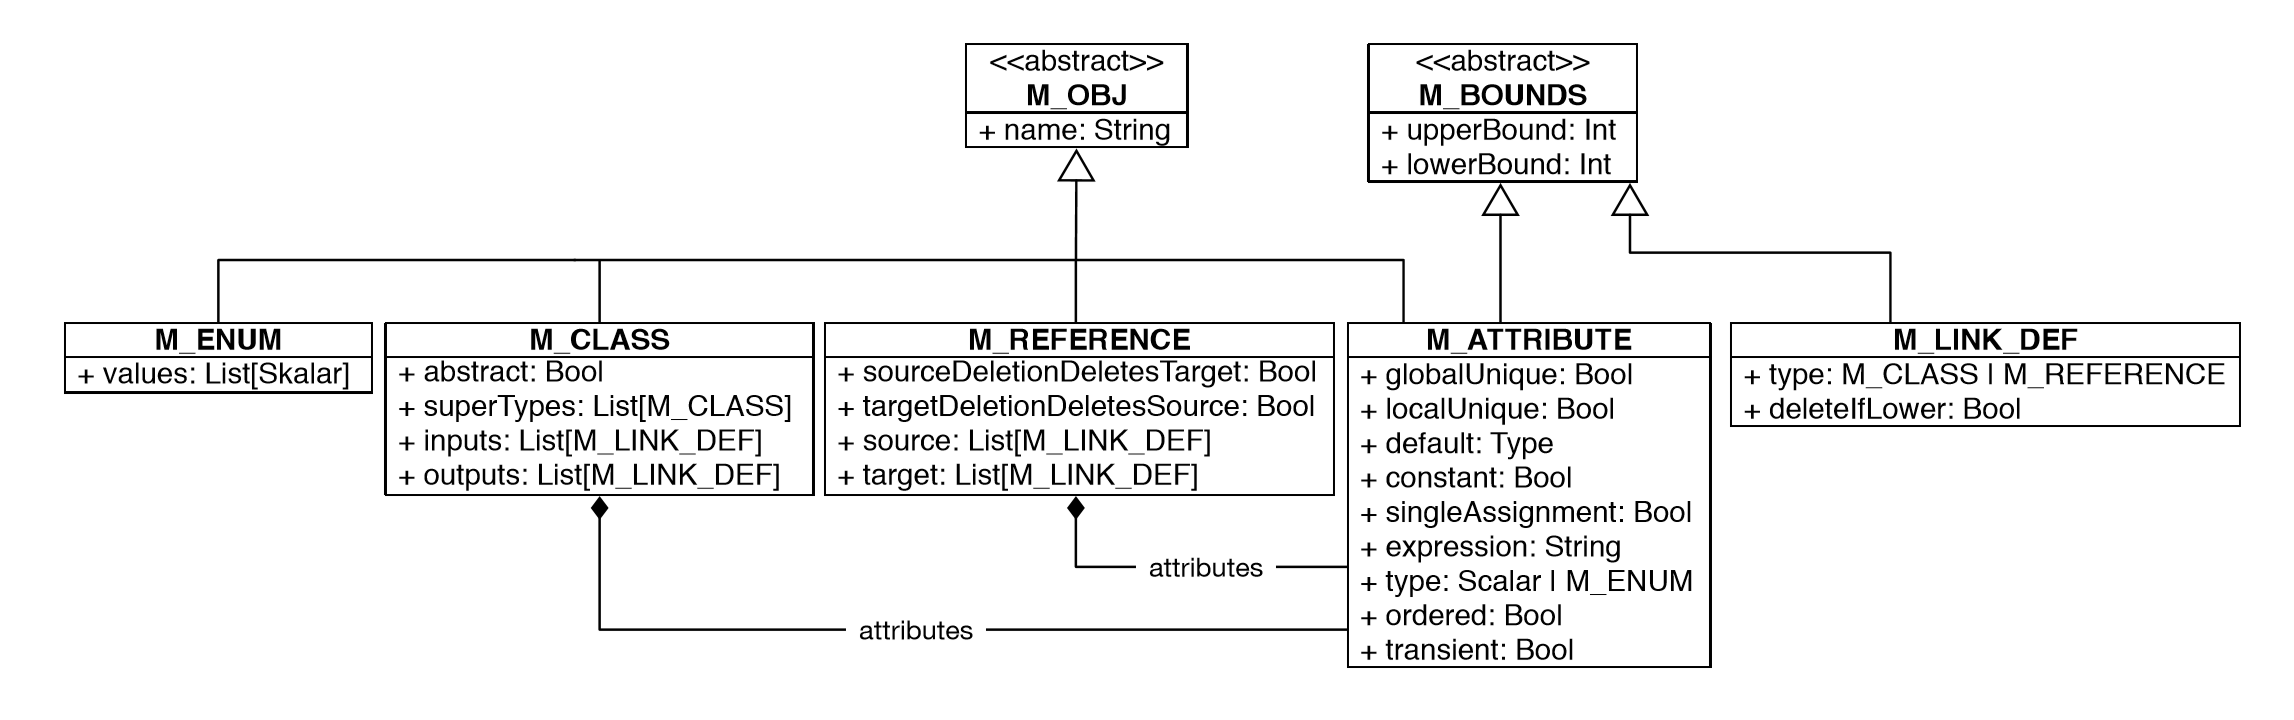
\includegraphics[width=\linewidth]{Abschnitte/Abbildungen/Grafiken/MoDiGen-Metamodel}
%
\epsfig{file=Quadrat.eps,height=1in,width=1in}
\caption{MoDiGen Metamodel}
\label{fig:MoDiGen-Metamodel}
\end{figure*}

Die abstrakte Klasse \textbf{M\_OBJ} enth\"alt das Attribut \textit{name}, dessen Wert innerhalb des gesamten Modells unikat ist. Dadurch wird es m\"oglich die erbenden Objekte zu identifizieren also die Instanzen von \textbf{M\_ENUM}, \textbf{M\_CLASS}, \textbf{M\_REFERENCE} und \textbf{M\_ATTRIBUTE}.
Eine Klasse mit ihren Attributen wird durch \textbf{M\_CLASS} und durch die Komposition zu \textbf{M\_ATTRIBUTE} im Modell erfasst. Vererbung wird durch das Attribut \textit{superTypes} modelliert. Hier ist anzumerken, dass auch Mehrfachvererbung dargestellt werden kann, da eine reflexive * Multiplizität vorliegt. 
Assoziationen werden durch \textbf{M\_LINK\_DEF} modelliert. Jede aus- bzw. eingehende Assoziation einer Klasse wird durch die Attribute \textit{inputs} und \textit{outputs} von \textbf{M\_CLASS} dargestellt, die auf \textbf{M\_LINK\_DEF} zeigen. Der \textit{typ} von \textbf{M\_LINK\_DEF} kann direkt eine \textbf{M\_CLASS} oder eine \textbf{M\_REFERENCE} sein. \textit{deleteIfLower} bestimmt, ob die enthaltende \textbf{M\_CLASS} bzw. \textbf{M\_REFERENCE} gel\"oscht wird sobald \textit{lowerBound} unterschritten wird. Um beliebige Multiplizitäten und Rollen zu beschreiben, wird \textbf{M\_REFERENCE} verwendet. Dazu besitzt diese Klasse die Attribute \textit{source} und \textit{target}, die jeweils beliebig viele Instanzen von \textbf{M\_LINK\_DEF} referenzieren können. Die Attribute \textit{lower-} und \textit{upperBound} von \textbf{M\_LINK\_DEF} bestimmen die Multitplizität. Um Assoziationsklassen \cite{larman2005book}[S. 290] zu modellieren kann \textbf{M\_REF\-ER\-ENCE} beliebig viele Referenzen zu \textbf{M\_ATTRIBUTE} besitzen. \textbf{M\_ENUM} erg\"anzt das Metamodell um Aufz\"ahlungstypen, die \"uber \textit{type} von \textbf{M\_ATTRIBUTE} verwendet werden k\"onnen.

\subsection{Beispiel}
Um das zugrundeliegende JSON-Format n\"aher zu beschreiben, wird im Folgenden als Beispiel ein vereinfachter Familienstammbaum verwendet (siehe Abbildung \ref{fig:Family-Tree-Model}).\\ 
Es existiert eine Entiät \textbf{Person}, die \textit{Vornamen}, \textit{Sozialversicherungsnummer} und \textit{Geburtstag} als Attribute besitzt. Die beiden Klassen \textbf{Male} und \textbf{Female} erben von \textbf{Person} und besitzen keine Attribute. Dabei kann \textbf{Male} eine Assoziation zu \textbf{Female} mit der Rolle \textit{isHusband} haben und, umgekehrt, die Klasse \textbf{Female} zu \textbf{Male} mit der Rolle \textit{isWife}. Das Eltern-Kind verh\"altnis wird durch 1:m Assoziationen von \textbf{Female} bzw. \textbf{Male} zu \textbf{Person} und der dazugeh\"origen Rolle (\textit{isMother}, \textit{isFather}) beschrieben.

\begin{figure}[H]
\centering
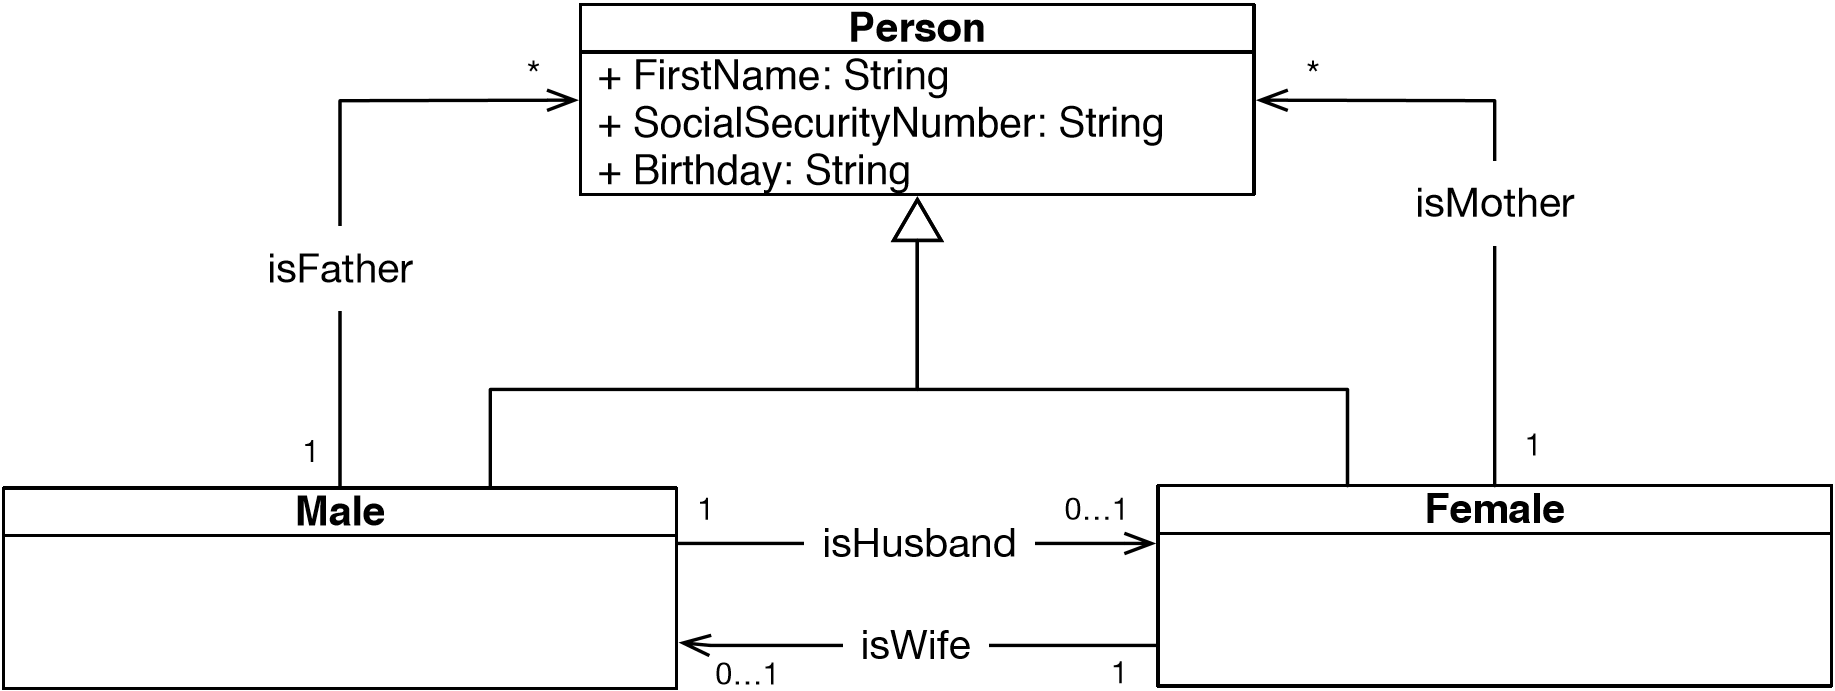
\includegraphics[width=\linewidth]{Abschnitte/Abbildungen/Grafiken/Family-Tree-Model}
\caption{Family Tree Model}
\label{fig:Family-Tree-Model}
\end{figure}


Die Klasse \textbf{Male} kann wie Listing \ref{lst:malejson} zeigt als JSON gespeichert werden. Dabei wird das JSON-Objekt \"uber den Klassennamen identifiziert -- hier \textit{Male} -- und durch das Attribut \textit{mType} als Klasse bestimmt. Da JSON keine implizite Typisierung unterstützt -- es unterscheidet lediglich zwischen wenigen generischen Datentypen -- muss hier explizit festgelegt werden, dass es sich um \textit{mClass} handelt. Die Assoziationen werden entsprechend als JSON-Arrays \textit{inputs} und \textit{outputs} gespeichert und enthalten die durch \textbf{M\_LINK\_DEF} definierten Attribute.

\lstlistingCode{M\_CLASS Male aus dem Family Tree Beispiel}{malejson}
"Male": { 
  "mType": "mClass", 
  "name": "Male",
  "superTypes": ["Person"], 
  "mAttributes": [], 
  "inputs": [{ 
    "type": "isWife", 
    "upperBound": 1, 
    "lowerBound": 0 
  }], 
  "outputs": [{ 
    "type": "isHusband", 
    "upperBound": 1,
    "lowerBound": 0 
    },{ 
    "type": "isFather", 
    "upperBound": -1,
    "lowerBound": 0
  }] 
}
\end{lstlisting}

Eine \textbf{M\_REFERENCE} wird als "`Objekt erster Klasse"' gespeichert wie Listing \ref{lst:ishusbandjson} zeigt und kann damit unabhängig von den \textbf{M\_CLASS} instanzen geladen werden. Das JSON-Objekt wird durch den Namen der \textbf{M\_REFERENCE} identifiziert und enth\"alt alle Attribute. Der Typ wird hier, wie bei \textbf{M\_CLASS} instanzen in \textit{mType} abgelegt. In den JSON-Arrays \textit{source} und \textit{target} werden, genau wie bei den \textbf{M\_CLASS} instanzen, die gesamten \textbf{M\_LINK\_DEF} instanzen abgelegt. In diesem Modell kann \textbf{Male} eine Assoziation der Rolle \textit{isHusband} haben. Diese \textbf{M\_LINK\_DEF} instanz zeigt auf die entsprechende \textbf{M\_REFERENCE} instanz, die wiederrum mit zwei Endpunkten zu \textbf{Female} und \textbf{Male} existiert. \textit{upper-/lowerBounds} sind hier jeweils 1, also wird der Sachverhalt "`Ein Ehemann ist der Mann einer Frau"' modelliert.

\lstlistingCode{Husband M\_REFERENCE Male aus dem Family Tree Beispiel}{ishusbandjson}
"isHusband": {
  "mType": "mRef", 
  "name": "isHusband",
  "mAttributes": [], 
  "source": [{ 
    "type": "Male", 
    "upperBound": 1, 
    "lowerBound": 1 
  }], 
  "target": [{ 
    "type": "Female", 
    "upperBound": 1, 
    "lowerBound": 1, 
  }] 
} 
\end{lstlisting}

Die Instanzen werden durch UUIDs identifiziert und enthalten Verweise auf ihre Typen im Modell sowie ihre Typen im Metamodell. Dies ist z.B durch die Kombination \textit{"`mClass"': "`Male"'} in Zeile 2 von Listing \ref{lst:instancejson} zu sehen. Es handelt sich um eine Instanz von \textbf{Male}, die wiederrum als Klasse, also als Instanz von \textbf{M\_CLASS} modelliert ist. Die \textit{outputs} und \textit{inputs} verweisen hier auf Instanzen von konkreten Referenzen -- in diesem Fall \textit{isHusband}, \textit{isWife} und \textit{isFather}.\\
Die Referenz \textit{isHusband} zeigt gem\"a\ss des Modells (Abbildung \ref{fig:Family-Tree-Model}) in \textit{source} auf eine Instanz von \textbf{Male} und in \textit{target} auf eine Instanz von \textbf{female}.

\lstlistingCode{Family Tree Instanz}{instancejson}
"846bc8a2-00fc-401f-b626-0b0252516aee": { 
  "mClass": "Male", 
  "outputs": { 
    "isFather": 
      ["8e9b1093-a589-4ae4-8e1e-1b3d63a3f842"], 
    "isHusband": 
      ["ee204744-6322-49d4-928e-1442e8bc70c4"] 
  }, 
  "inputs": { 
    "isWife": 
      ["666d4de7-e0f2-4620-8c19-d5469b40be1f"] 
  }, 
  "mAttributes": { 
    "First_Name": ["Hans"], 
    "SocialSecurityNumber": ["12"], 
    "Birthday": ["12-02-2015"] 
  } 
}, 

"ee204744-6322-49d4-928e-1442e8bc70c4": { 
  "mRef": "isHusband", 
  "source": { 
    "Male": 
      ["846bc8a2-00fc-401f-b626-0b0252516aee"] 
  }, 
  "target": { 
    "Female": 
      ["a264a43b-6f97-4257-9243-baddbf745490"] 
  } 
} 
\end{lstlisting}











\section{Evaluation} \label{sec:evaluation}
Es gibt verschiedene Metamodelle 

\section{Fazit und Ausblick}
Das hier vorgestellte Metamodell MoDiGen ist ein neuer Ansatz im Bereich DSML und bietet neue Möglichkeiten bei einem geringeren Speicherplatzbedarf. Die Art der Speicherung von Kanten als eigenständige Objekte ermöglicht neben der Speicherplatzreduzierung einen direkten programmatischen Zugriff auf die Kanten. Dies lässt aber auch zu, dass Kanten verwaisen können, indem ihre dazugehörigen Knoten gelöscht werden. Deshalb muss der jeweilige Modellierer angeben, ob eine Kante automatisch mit den dazugehörigen Knoten gelöscht wird. In Ecore hingegen werden die Kanten eines Knoten direkt mitgelöscht.\\
Das JSON-Format benötigt weniger Speicherplatz als XML-Format und erlaubt eine Darstellung auf Webseiten. Darüber hinaus können weitere Anpassungen und Speicherplatzoptimierungen in Javascript durchgeführt werden, um die Skalierbarkeit zu verbessern. \\
Dies sind die Neuerungen und Vorteile von MoDiGen gegenüber  anderen DSML-Tools. Neben den genannten Vorteilen gibt es noch einen weiteren Unterschied zu Ecore. In Ecore können zusätzlich zu Knoten und Kanten Operationen mit \texttt{EOperation} zu definiert werden. Dies ist aber nur ein Platzhalter der im Eclipse Modeling Frameworks implementiert werden kann. MoDiGen bietet diese Möglichkeit nicht. \\


\pagebreak
\rule{0.45\textwidth}{0.4pt}
\pagebreak
\rule{0.45\textwidth}{0.4pt}
\pagebreak


\section{Hinweise zu den folgenden Abschnitten}
Nach der Einleitung sollte in den folgenden Abschnitten der Inhalt des Papers vorgestellt werden. Die Einteilung der Abschnitte kann sich dabei am Paper orientieren.

\section{Hinweise zur Formatierung}
Ein paar Beispiele zur Formatierung von Text:
\begin{enumerate}
\item \textit{kursiv}
\item \textbf{fett}
\item \texttt{Code}
\end{enumerate}

\section{Tabellen}
\begin{table} % Einleitung der Tabelle
\centering % Überschrift zentriert
\caption{Ein paar Java-Schlüsselwörter} % Überschrift
\label{tab:example} % Label für spätere Referenzierung per \ref
\begin{tabular}{|c|c|} \hline % Einleitung des Tabelleninhalts
Schlüsselwort & Bedeutung \\ \hline % Zeile 1; Spaltentrennung per &
\texttt{abstract} & Abstrakte Klasse/Methode \\ \hline % Zeile 2
\texttt{class} & Einleitung einer Klasse \\ \hline % Zeile 3
\texttt{throw} & Exception werfen \\ \hline % Zeile 4
\end{tabular}
\end{table}

Tabellen lassen sich mit Hilfe der \texttt{table}- und \texttt{tabular}-Umgebungen setzen. Als Beispiel für eine konkrete Anwendung siehe Tabelle \ref{tab:example}.

Warum ist meine Tabelle nicht dort, wo ich sie definiert habe? Weil die Vorlage den "`floating"'-Modus von \LaTeX verwendet und Tabellen, Abbildungen und andere Elemente so anordnet, dass wenig Leerzeilen entstehen.

Die Positionierung der Elemente sollte dabei nicht manuell geändert werden, außer es handelt sich um doppespaltige Tabellen, Abbildungen etc. Ein Beispiel für ein doppelspaltiges Element zeigt Abbildung \ref{fig:doppelspaltig}.

Doppelspaltige Elemente werden durch Varianten der einleitenden Befehle mit dem Suffix "`*"' gesetzt:
\begin{itemize}
\item Tabellen: \texttt{begin\{table*\}}
\item Abbildungen (siehe Abschnitt \ref{sec:figures}): \texttt{begin\{figure*\}}
\end{itemize}

\section{Abbildungen}
\label{sec:figures}
Abbildungen werden durch die \texttt{figure}-Umgebung gesetzt. Als Format empfiehlt sich PostScript (ps) oder Encapsulated PostScript (eps).

\begin{figure}
\centering

\epsfig{file=Quadrat.eps,height=1in,width=1in}
\caption{Ein einspaltiges graues Quadrat (eps-Format).}
\end{figure}

\begin{figure*}
\centering

\epsfig{file=Quadrat.eps,height=1in,width=1in}
\caption{Ein doppelspaltiges graues Quadrat (eps-Format).}
\label{fig:doppelspaltig}
\end{figure*}

\section{Verweise}
Mit Hilfe von \LaTeX \ lassen sich eine Reihe von Verweisen auf weiterführende Informationen nutzen.

Die wichtigste "`Verweistechnik"' ist der Literaturverweis. Der Befehl für einen Literaturverweis lautet \texttt{\textbackslash cite\{<Bib\TeX-MARKE>\}}. \texttt{<Bib\TeX-MARKE>} ist dabei durch die jeweilige Bib\TeX-Marke zu ersetzen. Bei Bib\TeX \ handelt es sich um ein Programm, mit dem sich Literaturverweise definieren lassen. Es bietet eine Anbindung an \LaTeX. Ein Beispiel für eine Bib\TeX-Datei ist "`literatur.bib"', die sich im selben Verzeichnis wie diese \texttt{.tex}-Datei befinden sollte. Der Befehl \texttt{\textbackslash cite\{latex\}} führt dann zu folgender Ausgabe: \cite{latex}.

Die Bib\TeX-Datei "`literatur.bib"' können Sie entweder mit einem Texteditor anpassen oder Sie nutzen ein Tool wie JabRef\footnote{\texttt{http://jabref.sourceforge.net}}. Fußnoten setzt man übrigens mit \texttt{\textbackslash footnote\{\}}.

\section{Formeln}
Eine große Stärke von \LaTeX \ ist das Setzen von Formeln. Formeln können \textit{inline} gesetzt werden, d. h. sie erscheinen im Fließtext: $\lim_{n\rightarrow \infty}x=0$.

Formeln werden entweder in zwei \$...\$ eingeschlossen (Kurzform) oder sind von \texttt{\textbackslash begin\{$x$\}}...\texttt{\textbackslash end\{$x$\}} umgeben mit $x\in\left\{ \mathtt{math\textrm{,}\:\mathtt{equation\textrm{,}\: displaymath}}\right\}$ (Langform).

Formeln können auch in abgesetzter Form erscheinen, undzwar...
\begin{itemize}
\item ... nummeriert (\texttt{equation}-Umgebung):
\begin{equation}
{n+1\choose k} = {n\choose k} + {n \choose k-1}
\end{equation}

\item ... nicht-nummeriert (\texttt{displaymath}-Umgebung):
\begin{displaymath}
|x| = \left\{ \begin{array}{rl}
 -x &\mbox{ falls $x<0$} \\
  x &\mbox{ sonst}
       \end{array} \right.
\end{displaymath}
\end{itemize} 


\section{Quellcode}
Ab und an muss auch Quelltext gesetzt werden. Dies geschieht mit Hilfe des \texttt{listings}-Pakets\footnote{\texttt{http://texdoc.net/texmf-dist/doc/latex/listings/\\listings.pdf}}. Listing \ref{lst:example} zeigt ein Beispiel für ein "`floating"'-Listing.

\begin{lstlisting}[float, caption=Beispiel eines Java-Listings, label=lst:example, language=java, basicstyle=\small, tabsize=4, showstringspaces=false, numbers=left, frame=single, keywordstyle=\bfseries]
public class Main {
	public static void main(String[] args) {
		System.out.println("Hallo Welt");
	}
}
\end{lstlisting}

\section{Abschnitt 8 (Blindtext)}
\lipsum[5-10]

\section{Abschnitt 9 (Blindtext)}
\lipsum[11-20]

\section{Abschnitt 10 (Blindtext)}
\lipsum[21-30]

\section{Abschnitt 11 (Blindtext)}
\lipsum[31-32]

\section{Related Work (Blindtext)}
\lipsum[33-37]

\section{Zusammenfassung (Blindtext)}
\lipsum[42-44]

%%%%%%%%%%%%%%%% Epilog-ANFANG
% Die folgenden Zeilen zwischen Epilog-ANFANG und Epilog-ENDE bitte nicht ändern.

% Neue Seite für das Literaturverzeichnis
\newpage

% Der voreingestellte BibTeX-Stil ist abbrv und sollte nicht geändert werden. Er führt dazu, dass die Quellenverweise durchnummeriert werden, was die Regel für wissenschaftliche Veröffentlichungen in den Naturwissenschaften ist.
\bibliographystyle{abbrv}
%%%%%%%%%%%%%%%% Epilog-ENDE

% Verweis auf die BibTeX-Datei. Diese sollte im gleichen Ordner wie die tex-Datei liegen. ACHTUNG: Der Dateiname ist ohne die Endung .bib anzugeben.
\bibliography{literatur}
\end{document}